\chapter{Introduction}

Christopher B. Anderson

\section{Global Change Ecology}

The form and function of the earth's ecosystems are rapidly changing. Agricultural lands are now the largest terrestrial biome in the world, occupying approximately 40\% of the land surface \cite{Foley2005-la, Springmann2018-nr}. This expansion occurred at the expense of the world's forests, exerting an exacting toll in the tropics. There was a net loss of 42 million hectares of forest between 2000 and 2010 in tropical countries, commensurate with a net gain of 36 million hectares in agricultural lands \cite{Fao2016-yn}. Roughly two-thirds of agricultural area is pasture for livestock, which comprises approximately 60\% of global mammalian biomass, significantly outweighing humans and wildlife, which comprise the remaining 36\% and 4\% \cite{Ramankutty2008-lc, Bar-On2018-vj}. Simultaneously, forested area is increasing across temperate and boreal systems, and it is unclear whether total global forest area is increasing or decreasing over decadal time scales \cite{ Hansen2013-oz, Song2018-qd}.

\begin{figure}[!ht]
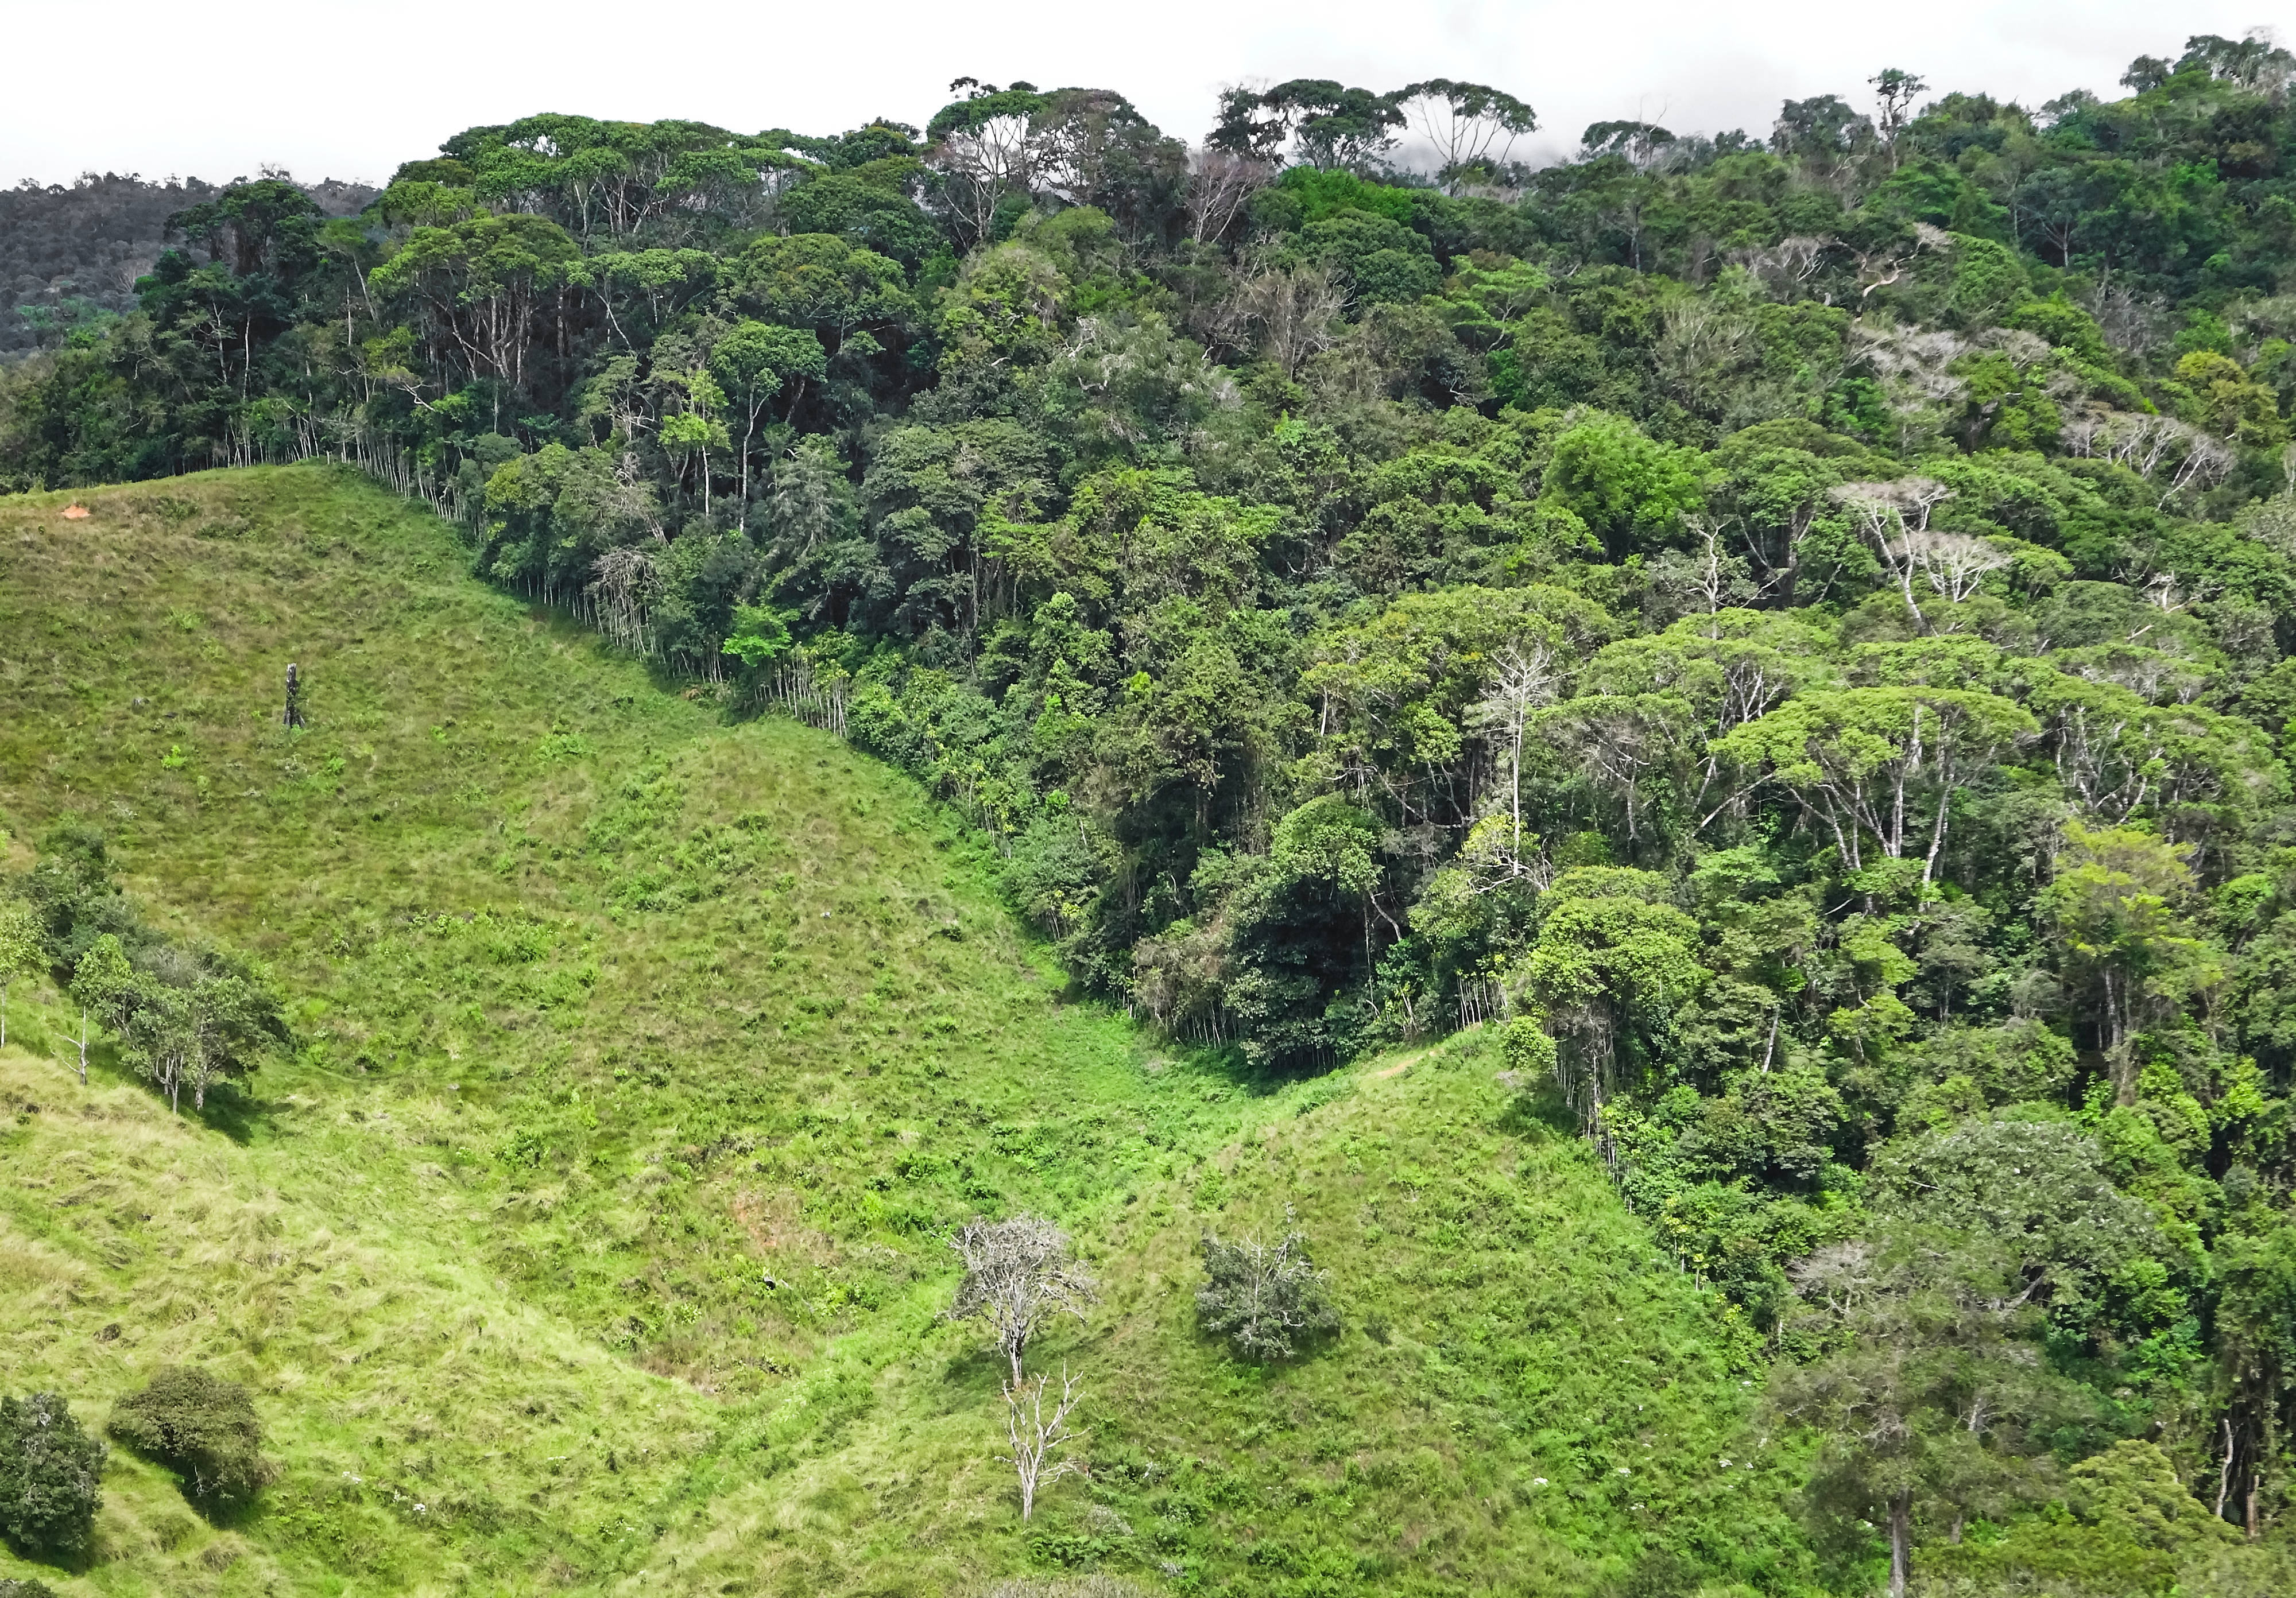
\includegraphics[width=\textwidth]{figures/intro-las-alturas.jpg}
\centering
\caption[Transition from forest to agriculture at the edge of the Las Alturas Wildlife Sanctuary in Costa Rica.]{Transition from forest to agriculture at the edge of the Las Alturas Wildlife Sanctuary in Costa Rica. Land use change is fundamentally altering patterns of ecosystem structure and ecosystem function, including the amount of wildlife habitat and patterns of primary productivity.}
\label{fig:las-alturas}
\end{figure}

This restructuring of the earth's ecosystems could be framed as a global game of whack-a-mole. Wildlife populations are crashing while livestock populations are booming. Forests are cut and cleared in the tropics, replanted and restored in temperate and boreal systems (Fig. \ref{fig:las-alturas}). This has had tremendous effects on terrestrial biodiversity; around 25\% of plant and animal groups are threatened, the extinction rate is now tens to hundreds of times higher than the average rate over the past 10 million years, and the number of invasive species per-country has increased nearly 70\%, all leading to the widespread erosion of differences between ecological communities \cite{IPBES2019-hl}. Ecosystems are a canonical example of complex, interconnected systems, and these changes are bound to have far-reaching consequences for other ecological processes. This includes the transmission of vector-borne diseases, which are poised to increase in frequency and intensity with environmental change, potentially exposing an additional billion people to the threat of Zika alone \cite{Ryan2020-ay}. With so much at stake, biodiversity monitoring systems are now being developed to track these complex patterns—the winners, the losers, the just differents—and to mitigate the effects of change.

A series of biodiversity monitoring frameworks have recently been developed to systematically assess change for multiple taxa over large extents \cite{Scholes2012-ec,Fernandez2015-na}. These monitoring frameworks have been shaped in large part by open access to biodiversity data \cite{Kattge2011-tf, Jetz2012-mw, Metzger2013-mz, Culina2018-ih} as well as access to an array of modeling tools to analyze these data \cite{Butchart2010-we, Pettorelli2016-wi, Gorelick2017-nx}. Most contemporary monitoring frameworks map biodiversity patterns according to the Essential Biodiversity Variables framework, a hierarchical grouping of metrics that quantify the variation in genes, species, communities and ecosystems \cite{Pereira2013-pk}. Inspired by the Essential Climate Variables framework, these metrics are i) biological, ii) sensitive to change, and iii) ecosystem agnostic, meaning they can be mapped anywhere. This definition is broad enough to include patterns of ecosystem structure, like aboveground biomass or habitat fragmentation, which are not often referred to as biodiversity \textit{per se}. This flexible and inclusive framework—which extends beyond a narrower definition of biodiversity as patterns of species richness, evenness and abundance—is now the standard for global monitoring systems, as it has been adopted by the intergovernmental Group on Earth Observations \cite{Geo_bon2017-ak}.

While the amount of open biodiversity data is now nothing short of incredible—the Global Biodiversity Information Facility (\url{https://www.gbif.org}) now hosts over 1.6 billion unique species occurrence records—the data gaps faced by monitoring systems are too wide to be bridged by \textit{in situ} biodiversity data alone. The spatial, taxonomic and temporal gaps in open biodiversity data are well documented \cite{Beck2014-am, Hortal2015-gc, Geijzendorffer2016-xv}, and a central task for the global biodiversity mapping community is to develop modeling approaches that address bias issues and extrapolate from incomplete records to map large extents.

Earth observations data, especially satellite imagery, are a natural compliment to \textit{in situ} data because they provide consistent measurements of terrestrial ecosystems over time, characterising biodiversity patterns in accessible and inaccessible areas alike. And plenty of data are available: at least 44 satellite constellations have been launched by 20 space agencies since 1977, which have been used to measure at least 15 different biodiversity patterns (Table B.1). But using satellites to map biodiversity is not a straightforward task. Satellites measure patterns of electromagnetic radiation, like spectral radiance, thermal emmissivity, or microwave backscattering, which are not in biological units of measurement. Given this fundamental difference in data types, it is worth reviewing the technical and conceptual basis for mapping biodiversity from earth observing sensors. How are satellite measurements converted from units of energy into metrics that are biological, sensitive to change, and ecosystem agnostic?

\section{Biodiversity Mapping with Earth Observations Data}

The majority of earth observing satellites are passive optical sensors that measure the amount of solar irradiance reflected by the earth's surface, typically in the spectrum of visible to shortwave infrared light (0.4-2.5 $\mu m$). Terrestrial vegetation, which covers the majority of the land surface, interacts with light in three ways. It absorbs light, with photosynthetic pigments harvesting photons to drive the electron transport chain and generate ATP. Vegetation also transmits light, often as a photoprotective mechanism to reduce potential molecular damage from harmful infrared radiation. The remaining light is reflected. This can be bidirectional, reflecting energy at an equal and opposite angle to the light source and normal to a leaf's surface, or it could be refracted and scattered spherically through the leaf tissue. The amount of light absorbed, transmitted, or reflected varies by wavelength and varies in response to many biophysical factors. Since most earth observing sensors measure reflected light, it is critical to understand the ecological processes driving vegetation reflectance patterns. Vegetation reflectance is driven by four general factors:

\begin{enumerate}
\item Leaf biochemistry, including the concentrations of pigments and defense compounds (Fig. \ref{fig:modeled-spectra}A).
\item Plant resource use, including leaf water content and nitrogen content (Fig. \ref{fig:modeled-spectra}B).
\item Leaf structure, including cell wall composition (e.g., cellulose and lignin concentrations) and the amount of intracellular air space (Fig. \ref{fig:modeled-spectra}C).
\item Canopy structure, including the number and orientation of leaves on a plant (Fig. \ref{fig:modeled-spectra}D).
\end{enumerate}

\begin{figure}[!ht]
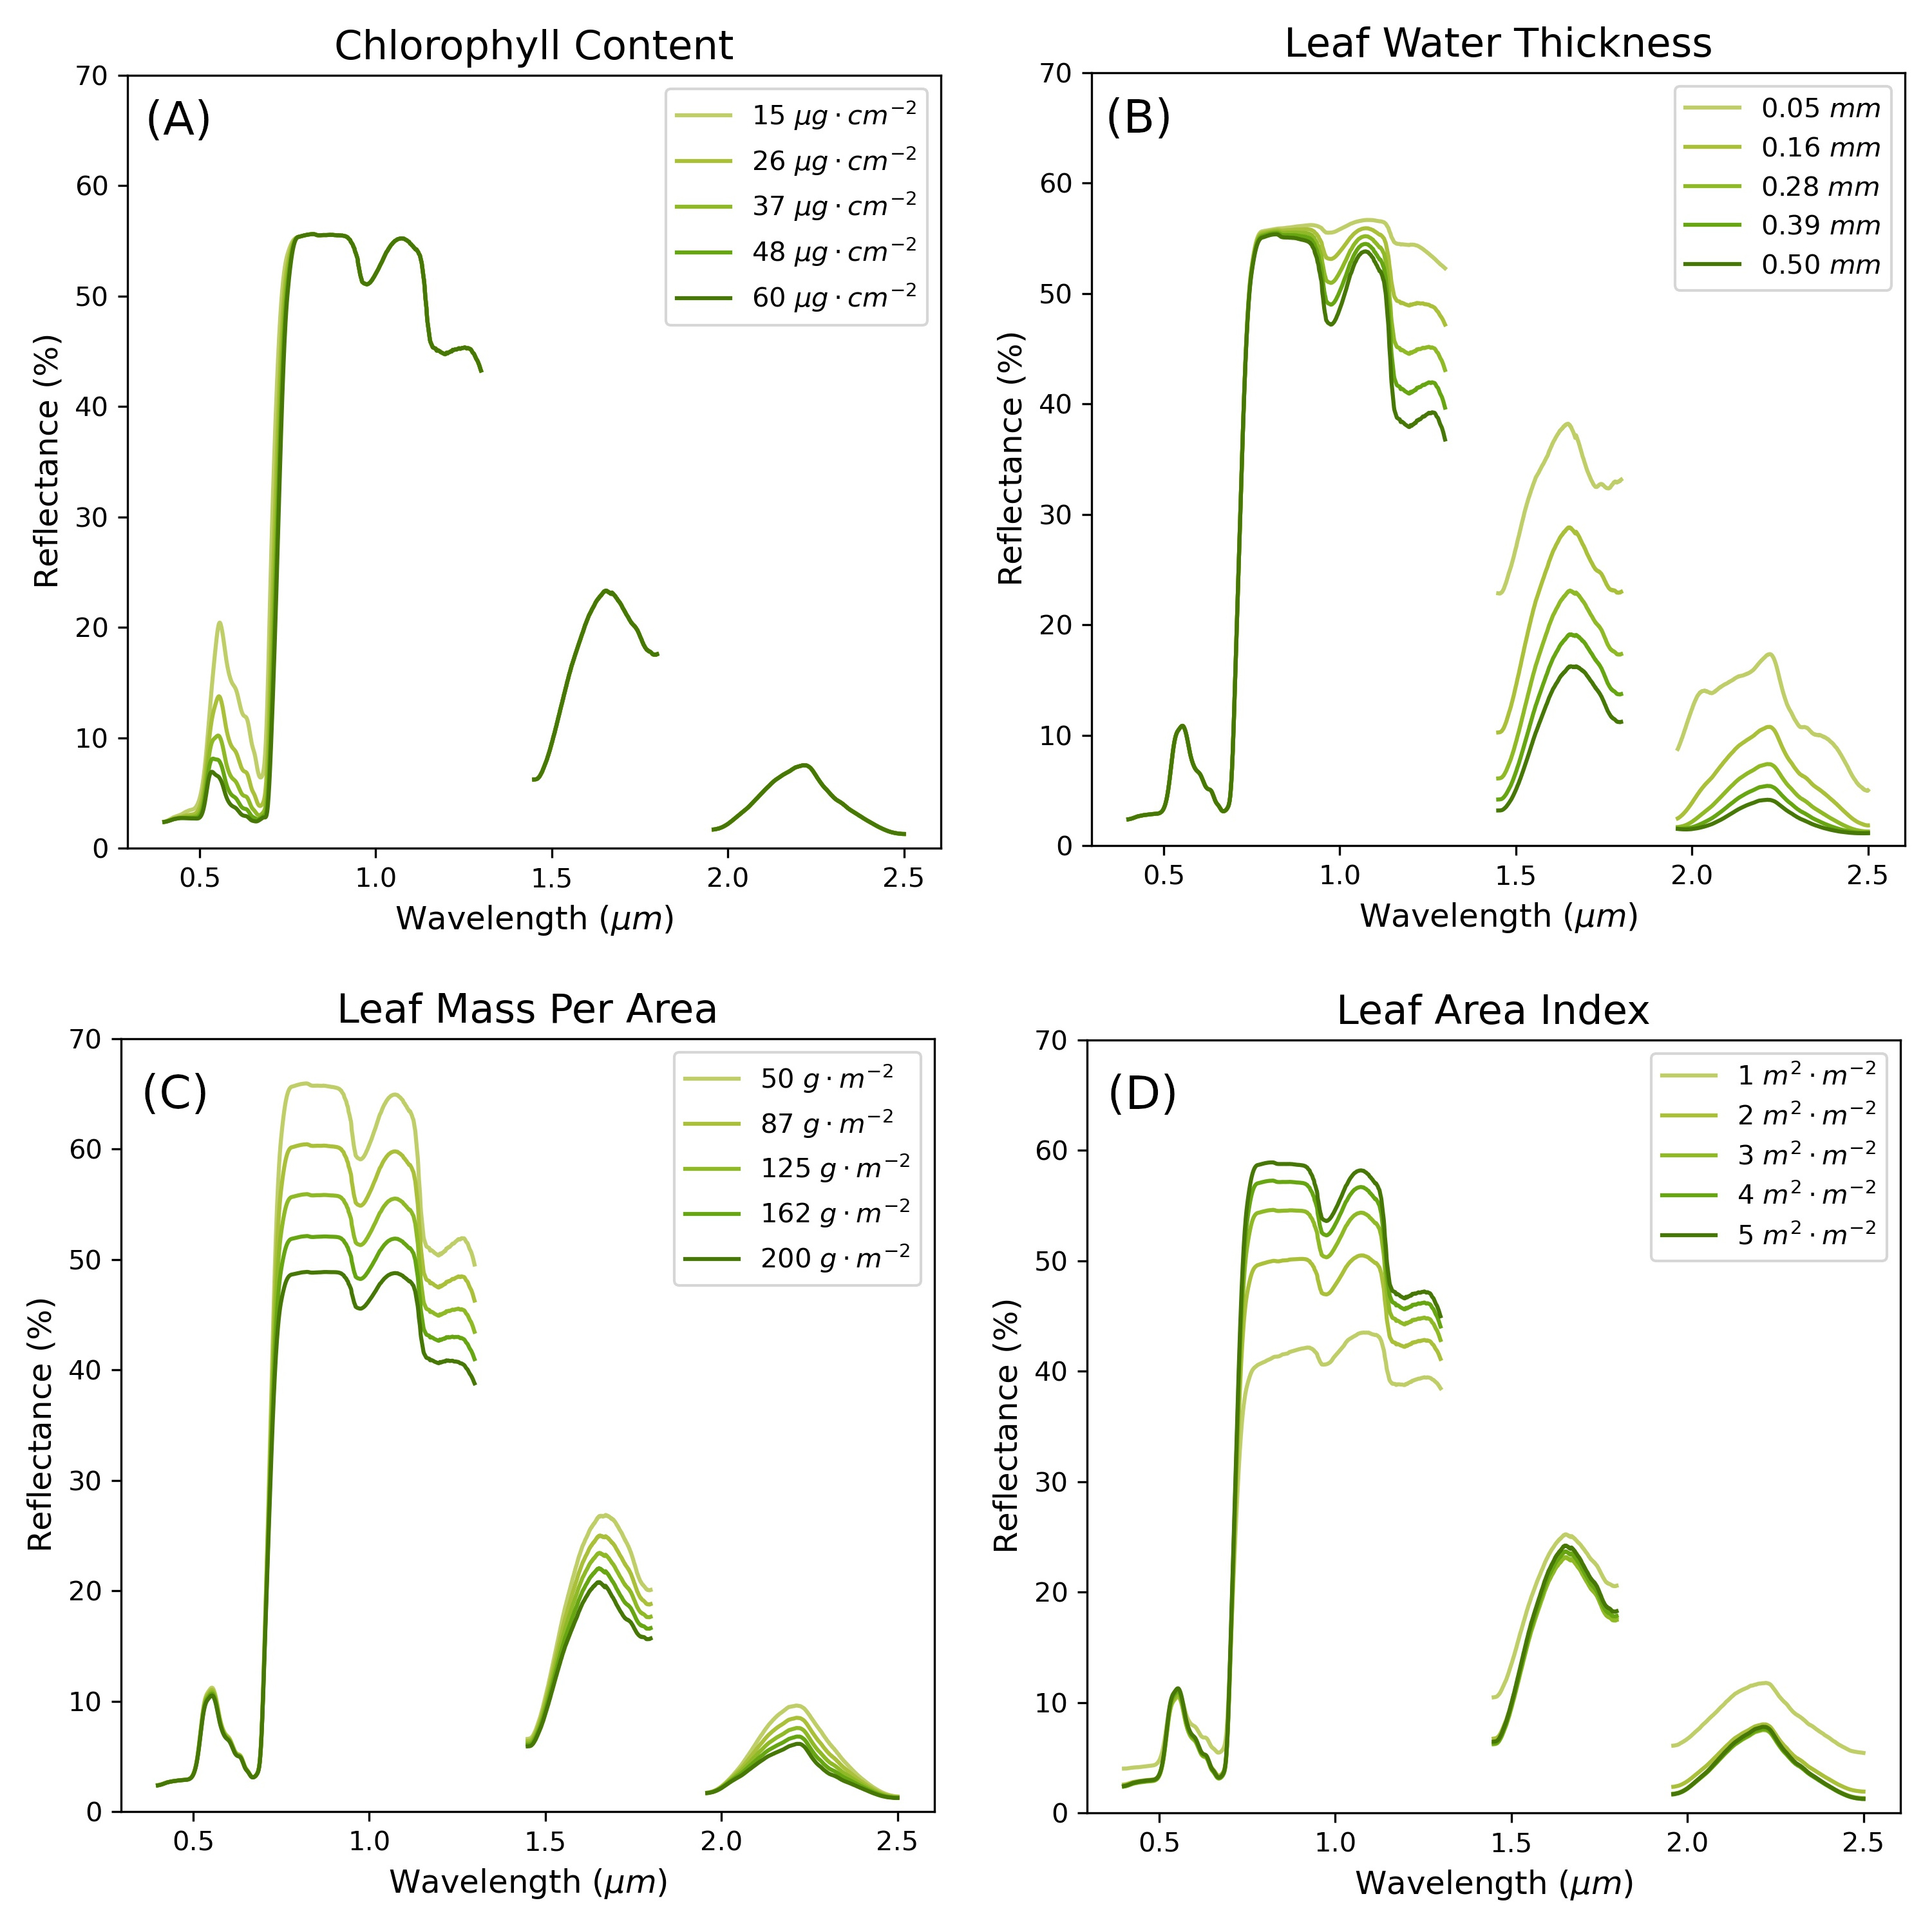
\includegraphics[width=\textwidth]{figures/intro-modeled-spectra.jpg}
\centering
\caption[Simulated vegetation reflectance spectra showing the nonlinear effects of variation in different leaf and canopy properties.]{Simulated vegetation reflectance spectra showing the nonlinear effects of variation in four leaf and canopy properties: (A) leaf chlorophyll content, (B) leaf equivalent water thickness, (C), leaf mass per area, and (D) leaf area index. All spectra were generated using the PROSAIL coupled leaf and canopy model \cite{jacquemoud2009prospect+} using a range of global parameter values \cite{Rivera2013-gq}. For (A)-(D), each parameter was set to the global mean, with the exception of the focal parameter, which varied in a range from min and max of the 95\% range. Bands dominated by atmospheric water vapor concentrations (1.3-1.45 $\mu m$  and 1.8-1.96 $\mu m$) were removed.}
\label{fig:modeled-spectra}
\end{figure}

This is also important in the context of biodiversity monitoring because these four factors are also indicators for discriminating between species. Plant biochemistry is well-conserved among individuals of the same species \cite{Kokaly2009-xk, Asner2011-tn, Funk2017-io}, as are resource use patterns and leaf and canopy structure patterns \cite{Halle1978-zu, Townsend2007-zm}. Interspecific variation in these patterns is driven by resource access, competition and co-evolution, leading to niche partitioning and differentiation along multiple niche axes \cite{Wright2004-md, Osnas2013-vp}. Reflectance patterns therefore contain information that could be used to classify species identities in sufficiently detailed optical data. The methods that decompose these signals to map species traits and identities, or patterns of ecosystem structure and function, are referred to throughout this work as methods for \textit{measuring} biodiversity patterns. Due to multiple forms of covariance—including covariance between traits as well as covariance from each trait propagating signal across the reflectance spectrum—disentangling the effects of each factor is a major challenge. \textit{Chapter 2} is a review of some of the scale-dependent challenges to signal decomposition in the context of biodiversity mapping, and \textit{Chapter 3} describes a machine learning method that overcomes some of these challenges through ecologically-informed data preprocessing to identify tree species in high resolution imagery.

In addition to passive optical sensors, there is a diverse array of earth observing sensors that measure other biologically and ecologically important patterns. Thermal sensors measure midwave (3-8 $\mu m$) and longwave (8-10 $\mu m$) emmissivity patterns, which can be used to map surface temperature patterns \cite{Li2013-uw}. Microwave instruments are sensitive to the volume of liquid or atmospheric water, depending on the sensor, tracking patterns ranging from precipitation to canopy water content \cite{Hou2013-cn, Konings2019-fd}. Even cloudy pixels in optical data, which make up around 60\% of observations and are generally a nuisance for biodiversity mapping, have been used to refine the extents of cloud forests and improve predictions of fog-dependent species distributions \cite{Wilson2016-pv}. 

These patterns are useful in biodiversity monitoring contexts despite violating the ``biological" requirement to be considered Essential Biodiversity Variables. Niche use patterns are often defined by temperature, precipitation, and cloud cover patterns, placing abiotic constraints on the spatial distributions of species (which are indeed biological, sensitive to change, and can be mapped across ecosystems). Since these measurements are often used as predictive features in spatial biodiversity models, these data are referred to throughout this document as useful for \textit{modeling} biodiversity patterns. \textit{Chapter 2} explores the scale-dependent challenges of modeling biodiversity patterns with earth observations data, and is especially concerned with species distribution modeling examples. \textit{Chapter 4} applies the lessons learned from those use cases to modeling the spatial distributions and niche use patterns of two globally-invasive mosquito arbovirus vectors, \textit{Aedes aegypti} and \textit{Ae. albopictus}, which are expected to continue expanding to new regions as temperature and precipitation patterns shift with climate change \cite{Tjaden2018-zi, Ryan2019-pz}.

\section{Dissertation Themes}

There are three general themes explored in this dissertation. First is regarding the role of spatial and temporal measurement scales in determining which biodiversity patterns can be detected by earth observations sensors, including what drives signal variance at each scale. Changing measurement scales, both by definition and in practice, changes the biological variation within and between measurements, and nonlinear patterns often emerge at ecological boundaries known as domains of scale. The transition from measuring leaf reflectance to measuring canopy reflectance is an example of these nonlinear effects. Light traveling through a canopy is absorbed, transmitted and reflected by individual leaves, and the transmitted and scattered photons can be absorbed, transmitted, or reflected by other leaves within the canopy. Since the amount of light absorbed, transmitted, or reflected varies by wavelength, plant canopies are spectrally distinct from the individual leaves that comprise them, with dense canopies absorbing more visible light and scattering and reflecting more infrared light. This is the mechanistic basis for retrieving forest structural patterns like leaf area index from optical data \cite{Jordan1969-ol}. While some changes propagate across scales, like changes in chlorophyll concentrations, the methods for measuring these changes depends on the scale of analysis, as canopy structure introduces additional spectral variance that covaries with pigment changes. Identifying the appropriate domains of scale for analysis is a critical when measuring and modeling biodiversity patterns, and the example above is explored in-depth in \textit{Chapter 3}.

The second theme of this dissertation concerns the Goldilocks principle. Considering the global nature of the field, ecology was previously a data-scarce discipline, as many central ecological theories were derived from data on a single species, a single community, or a few islands \cite{Grinnell1917-aa, Hubbell2001-lq, MacArthur1967-zp}. The past decade has upended this trend, as open and standardized biodiversity data are more abundant and accessible than ever. So, too, are global earth observations data. But this flood of information can be overwhelming. This dissertation explores approaches to combining incomplete species data (``too little") with abundant earth observations data (``too much") to map patterns of biodiversity that are ``just right." \textit{Chapter 3} decomposes 426 spectral reflectance bands from airborne imaging spectroscopy data into principal components finding that, with feature selection, only around 20-30 components were required to discriminate between species. \textit{Chapter 4} analyzes over 8,000 species occurrence records and distills 16 years of daily satellite imagery into descriptive metrics of climate, habitat and resource use across Latin America and the Caribbean to quantify constraints on niche use for \textit{Ae. aegypti} and \textit{Ae. albopictus}, mapping the potential distributions of these arbovirus disease vectors at continental scales.

The final theme of this dissertation is the use of biomimicry: selecting and training machine learning models to approximate mechanistic ecological models. Commensurate with the expansion of open data, machine learning methods for analyzing ecological data have recently proliferated \cite{Pal2005-qh, Phillips2006-ua, Hastie2009-fs, Elith2011-kb, Brodrick2019-jz}. These are essential tools for identifying novel patterns in large datasets where mechanistic relationships are unclear. But they are also prone to overfit to spurious, non-biological patterns, especially in spatial contexts \cite{Hawkins2012-gu, Fourcade2018-ws}. I approach the problem in this dissertation by carefully selecting machine learning models that mimic well-known ecological processes, using data that has been transformed to fit model assumptions. \textit{Chapter 3} uses decision tree ensembles to predict tree species identities based on decomposed reflectance data, approximating a dichotomous tree and morphological trait-based taxonomy. \textit{Chapter 4} fits non-linear and smoothly varying response functions to climate, habitat, and resource use patterns for \textit{Ae. aegypti} and \textit{Ae. albopictus}, which was designed to mimic thermal response functions characterized for those vectors in laboratory settings \cite{Mordecai2019-ya}.

Together, this work further develops the technical and conceptual basis for building biodiversity monitoring systems that carefully integrate earth observations and \textit{in situ} data. However, much work remains to actually build these systems and provide the data to the right stakeholders who can use it to inform conservation and land management decisions \cite{Guerry2015-zt, Ramirez-Reyes2019-nq}. The end of the last decade marked the time to deliver on the promises of the Ecosystem Services framework; now is the time to deliver on the promise of biodiversity monitoring \cite{Daily2009-jz, IPBES2019-hl}.

\clearpage

\section{Publication and Copyright Notices}

Two of the following chapters have been published in peer-reviewed journals under open-access licenses. Chapter 2 was published in \textit{Ecology Letters} in July 2018, which is reprinted with permission from the publisher, John Wiley and Sons Ltd. The full license agreement is included in \textit{Appendix D}. The full citation is:

\begin{quote}
    Anderson, C. B. (2018). Biodiversity monitoring, earth observations and the ecology of scale. \textit{Ecology letters}, 21(10), 1572-1585.
\end{quote}

\noindent Chapter 3 was published in \textit{PeerJ} in October 2018 with the following full citation:

\begin{quote}
    Anderson, C. B. (2018). The CCB-ID approach to tree species mapping with airborne imaging spectroscopy. \textit{PeerJ}, 6, e5666.
\end{quote}

\noindent Per the \textit{PeerJ} Copyright Policy (\url{https://peerj.com/about/policies-and-procedures/}):

\begin{quote}
    All \textit{PeerJ} articles are published under a Creative Commons Attribution License. With this license, Authors retain copyright, but allow any user to share, copy, distribute, transmit, adapt and make commercial use of the work without needing to provide additional permission, provided appropriate attribution is made to the original author or source.
\end{quote}

\noindent Chapters 1, 4, and 5 are currently unpublished outside of this dissertation.